%============================================================================%
% Author: Pablo S�nchez                                                      %
%         p.sanchez@unican.es, http://personales.unican.es/sanchezbp         %
% Section : Research Challenges                            Date: 25/02/2011  %
% Version : 1.0                                                              %
% Conference: SPLC 2011                                                      %
%============================================================================%

%============================================================================================
% NOTE(Pablo): This is not required for SPLC 2011
%============================================================================================
%
% The creation of clonable features was initially an easy task, since it only required to add
% the notion of cardinality to each feature. Nevertheless, this has created several
% side-effects, since some concepts such as the semantics of a clonable feature selection, had % to be reviewed and updated. This section identifies several problems, not currently solved to % the best of our knowledge, regarding the specification of external constraints involving
% clonable features.
%
%============================================================================================

%============================================================================================
% NOTE(Pablo): Too much verbose
%============================================================================================
%
% Nevertheless, this had several consequences, since it was required to review an update
% well-established concepts related to feature modelling and to answer several research
% challenges that emerged as a consequence of introducing this new concept. Previous section
% described how clonable features are selected by means of a new cloning operation. This
% section identifies several problems, not currently solved to the best of our knowledge,
% regarding the specification of external constraints between features when some of the
% features involved in the constraint are clonable.
%
%============================================================================================

Clonable features creates new challenges when the specification of cross-tree constraints is required. For instance, according to Figure~\ref{fig:smartHomeFM}, house facilities can be selected at a house, floor or room level. Therefore, a cross-tree constraint should specify if \imp{LightMng} has been selected at the floor level, this facility must also have been selected for each room belonging to that floor.

Since \imp{SmartEnergyMng} requires the \imp{HeaterMng} and \imp{WindowMng} features have been selected, other constraint should specify whenever \imp{SmartEnergyMng} has been selected at one level (e.g. for a specific floor), \imp{HeaterMng} and \imp{WindowMng} have also been selected at the same level (i.e. for that specific floor). Finally, we might want to specify more advanced constraints, like if \imp{Presence Simulation} is going to be included in a automated house, a 25\% of the rooms in the house at least must include automatic light management .

In feature models, the most usual way to express cross-tree constraints is using propositional logic formulas, such as \imp{SmartEnergyMng implies (LightMng and HeaterMng)}, where the different features are the atoms for these formulas~\cite{batory:2005}. An atom is evaluated to true when the corresponding feature has been selected, otherwise it is false. The main problem when dealing with clonable features is that this correspondence cannot be used. Clonable features are not selected or unselected. Clonable are just cloned. So, the meaning of a atom related to a clonable feature becomes undefined. As a result, a propositional logical formula including clonable features can not be evaluated and it can not be determined when the corresponding constraint has been satisfied or violated.

For instance, let us suppose  \imp{A} and \imp{B} are clonable features. In this case, what would be the meaning of a external constraint like \imp{A implies B}? Does this means that one instance of \imp{A} implies the existence of at least one instance of \imp{B}? Or, on the other hand, does it means that the existence of all potential \imp{A}s implies the existence of all potential \imp{B}s? Or, why not, the existence of all potential \imp{A}s implies the existence of only one \imp{B}? So, the first research challenge we face is to decide what a clonable feature exactly means in a logical formula expressing a cross-tree constraint.

Each clonable feature really evaluates to a set of clones. For instance, the feature \imp{Floor} in Figure~\ref{fig:smartHomeFM} actually evaluates to \imp{\{Ground, First \}}, instead of selected or unselected. Thus, we might want to specify properties that only applies to: (1) at least one element in that set (e.g. only to the \imp{Ground} floor); (2) to all the elements in that set that fulfill a certain constraint (e.g to all the floors with \imp{LightMng} selected in one room at least); or (3) all the elements in the set. This would allow us to express more complex constraints such as, such as: if \imp{HeaterMng} is selected per house level, one \imp{Room} at least must contain one \imp{Heater} as a minimum. So, our second research challenge is to add quantification mechanisms to constraints involving clonable features.

%============================================================================================
% TODO(Pablo): Redo this image using Hydra. It is quite hard to get Hydra working for this
%              purpose
%============================================================================================

\begin{figure}[!tb]
  % Requires \usepackage{graphicx}
  \centering 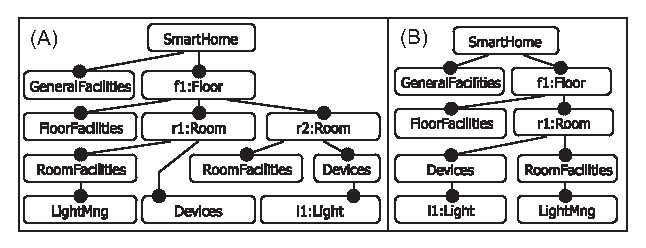
\includegraphics[width=\linewidth]{Figures/contexts.eps} \\
  \caption{(Left) Invalid configuration (Right) Valid configuration}
  \label{fig:contexts}
\end{figure}

Moreover, as already commented in previous section, we might want to specify constraints which must be evaluated for a particular subtree of the whole feature model, i.e. in a particular \emph{context}. For instance, if \imp{LightMng} has been selected for a particular \imp{Room}, such a \imp{Room} must have one \imp{Light} at least. Thus, we should specify a constraint like ``\imp{LightMng} implies one \imp{Light} device at least''. If we do not limit the scope in which this constraint is evaluated, this constraint will be true for the configurations of Figure~\ref{fig:contexts} (a) and (b). Nevertheless, this constraint should be false for Figure~\ref{fig:contexts} (a), since \imp{r1:Room} has selected the \imp{LightMng} facility, but it has not any \imp{Light} device to control. This means this constraint must be evaluated for all rooms (notice we are using again quantification) and using only the subtree below each \imp{Room}. Thus, the third research challenge is how to specify and analyse constraints which must be must be evaluated in the scope of a particular context.

%============================================================================================
% NOTE(Pablo): Since we have opted for leaving out feature references, this paragraph must
%              also be left out of the paper.
%============================================================================================
%
% Contexts are also useful for solve ambiguities when using feature references, since multiple % copies of a same feature might appear at different part of a configuration model. For
% instance, does \imp{LightMng} refers to \imp{LightMng} for \imp{GeneralFacilities},
% \imp{FloorFacilities} or \imp{RoomFacilities}. Using contexts, we can limit the scope of a
% name to unambiguously refer to a certain feature.
%
%============================================================================================

Finally, we would to like to point out that not only clonable features can have more than one instance per configuration of a feature model. All those features that have as an ancestor a clonable features can appear more than once in a configuration model. We will call to this kind of feature, i.e. non clonable features with a clonable ancestor, \emph{multiple features}.
Figure~\ref{fig:multipleFtr} illustrates this situation.In this case, the feature \imp{LightMng} below \imp{RoomFacilities} appears two times due to the \imp{Room} feature has been cloned twice. This implies that \imp{LightMng}, as well as the other features below \imp{Room}, also evaluate to a set of features instead of simply to true or false. Nevertheless, it should be noticed that these multiple features, oppositely to clonable features, can be evaluated to true or false if they are evaluated in a particular context.
For example, the \imp{LightMng} feature in Figure~\ref{fig:multipleFtr} can be evaluated to true or false when it is evaluated in the context of a particular room. So, our last research challenge is how to deal appropriately with \emph{multiple features}.

\begin{figure}[!tb]
  \centering 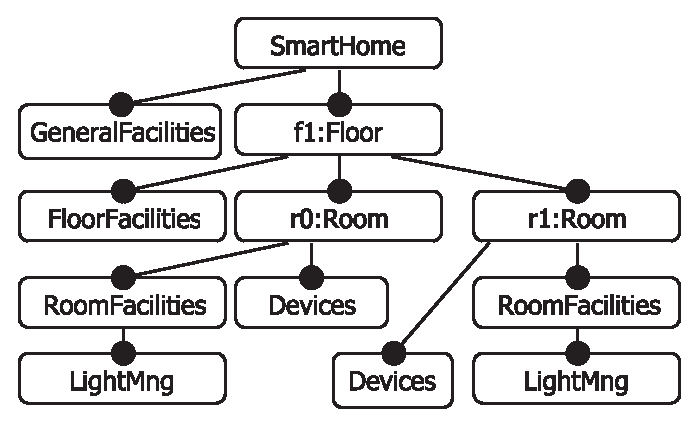
\includegraphics[width=.65\linewidth]{Figures/multipleFeatures.eps} \\
  \caption{The \emph{multiple features} phenomena}
  \label{fig:multipleFtr}
\end{figure}

Summarising, when dealing with clonable features, we should to address the following research challenges to properly express and analyse cross-tree constraints between features:

\begin{enumerate}
	\item What a clonable feature means in a cross-tree constraint.
	\item Add quantification mechanisms to cross-tree constraints.
	\item Add the notion of \emph{context} to cross-tree constraints.
	\item Manage properly multiple features.
\end{enumerate}

To the best of our knowledge, there is currently no research work, and consequently no tool, addressing these challenges. To overcome this limitation, we have firstly created a language for expressing arbitrary complex constraints including clonable features as a stepping stone towards the analysis of constraints including clonable (or multiple) features. Next section describes sauch a language.

%============================================================================================
% NOTE(Pablo) : This have been supressed because it sounds redundant
%============================================================================================
%
% We have implemented a reasoner able to decide if a set of external constraints, involving
% clonable or multiple features, is satisfied given a specific configuration of a feature
% model. The reasoner is also able to perform some extra task, such as deciding which features % must be incorporated to a configuration in order to satisfy the external constraints. We have % integrated this language and the reasoner in our feature modelling environment, which we have % called \emph{Hydra}.
%
%============================================================================================

%============================================================================================
% NOTE(Pablo) : We have reduced this paragraph. We are no presenting a tool, so this
%               paragraph can be simply skipped
%============================================================================================
%
% State-of-art tools only offer two operators, \imp{implies} and \imp{excludes}, and deal with % simple propositional formulas. This is clearly not enough to address the research challenges % described in this section.
%
%============================================================================================

%=============================================================================================
% NOTE(Pablo): This paragraph would be suitable for a very general venue                                                                                 %=============================================================================================
%
% A typical feature modelling process would be as follows:
%
% \begin{enumerate}
%    \item First of all, a feature model is created. A feature model is a tree representation
%          of the features included in % a set of products and of the relationships between
%          them.
%    \item Since not all the relationships between features can be captured using simply the
%          syntax provided by feature  models, it is often required to specify some external
%          constraints, which restrict the way in which features in a feature model can be
%          selected. For instance, we might specify that if a certain feature \imp{A} is
%          selected, another feature \imp{B} can not be selected, due to a bad interaction
%          between these features.
%    \item Once we have created a feature model, we can use it for creating configurations,
%          i.e. selection of features that specify which particular features are, or it will
%          be, included in a certain product.
%    \item To ensure we are creating correct configurations, we need to validate that a
%          configuration obeys the rules the % syntax of the feature model, and, in addition,
%          it also satisfies the external defined constraints.
% \end{enumerate}
%
%=============================================================================================

